\documentclass[11pt]{article}

\usepackage[margin=1.15in]{geometry}
\usepackage{amsmath}
\usepackage{amssymb}
\usepackage{graphicx}

% Floats: no page may hold only a figure with the rest blank.
\renewcommand{\topfraction}{0.9}
\renewcommand{\bottomfraction}{0.8}
\renewcommand{\textfraction}{0.07}
\renewcommand{\floatpagefraction}{0.85}
\setcounter{topnumber}{3}
\setcounter{totalnumber}{4}

% One symbol per object, as in notes/fog_parameter_degeneracy_study.
\newcommand{\kmax}{k_{\rm max}}
\newcommand{\hMpc}{\,h/{\rm Mpc}}
% The unit of the counterterms.
\newcommand{\aunit}{\,h^{-2}\,{\rm Mpc}^2}
% The UV-fraction threshold.  Written with its subscript everywhere,
% so it never collides with the counterterms alpha_0 and alpha_2.
\newcommand{\auv}{\alpha_{\rm UV}}
% The reference layout, as the reader-facing text names it.
\newcommand{\dcom}{$\Delta d_{\rm com} = 62$~Mpc}
% An underscore after which a long code name may break.
\newcommand{\us}{\_\allowbreak}
% The clause every caption that quotes k_max carries.
\newcommand{\kmaxclause}{$\kmax$ quoted at $z = 0$; each bin is cut at
  $\kmax/D(\bar{z}_i)$.}

\title{How much does the scale cut depend on its fiducial?}
\date{November 2026}
\author{}

\begin{document}

\begin{center}
  {\LARGE How much does the scale cut\\[0.3em]
    depend on its fiducial?\par}
  \vspace{0.6em}
  {\large The UV-fraction cut computed on the linear-bias fiducial
    against\\ the paper model's own, in kept band powers and figures
    of merit\par}
  \vspace{1em}
  {\large November 2026\par}
\end{center}
\vspace{1em}

\section{Summary}
\label{sec:summary}

\paragraph{The question.}
The forecast removes small scales with the UV-fraction cut of
Saraivanov et al.~\cite{Saraivanov2026}: a band power is kept while
less than five percent of it comes from modes above a redshift-scaled
wavenumber threshold (Section~\ref{sec:cut} defines every
ingredient).  Because the cut splits the \emph{model's own} spectra,
it must be computed on some model at some parameter point -- a
fiducial, the single point in parameter space at which a forecast is
evaluated.  The forecast computes the cut on the model it analyzes.
The paper notebook computes it on the paper model's fiducial -- the
fiducial model: one-loop galaxy bias with per-group offsets and
tilts, the line-of-sight
counterterm $\alpha_2$ fixed at zero and the Fingers-of-God
dispersion priors widened by a factor of six.  The linear-bias
experiments keep a cut computed on the linear fiducial, where each
bin carries only its linear galaxy bias $b_1$ (the coefficient
relating the galaxy density contrast to the matter one on large
scales).  This note measures what that consistency is worth: how much
the cut, and the science downstream of it, move between the two
fiducials.

\paragraph{The answer.}
\begin{enumerate}
  \item \textbf{The two fiducials differ in exactly two numbers per
    bin.}  At the paper model's fiducial point every parameter beyond
    linear bias is either zero (the counterterms, the stochastic
    terms, magnification) or shared with the linear fiducial (the
    cosmology, $b_1$, the dispersions, redshift-space distortions).
    What remains are the second-order biases $b_2$ and $b_{s^2}$,
    sitting on their calibration relations
    (Section~\ref{sec:sees}).
  \item \textbf{The cut moves by about one band per affected
    spectrum.}  The kept band powers change by $1$--$3\%$ at
    $\kmax \le 0.1\hMpc$ on every layout
    (Figure~\ref{fig:kept}).  Auto spectra only lose bands, almost
    always one; cross-bin pairs move both ways, and a few pairs whose
    spectra change sign swing by tens of bands at
    $\kmax \ge 0.175\hMpc$ under either fiducial.
  \item \textbf{The science moves less.}  The paper model's
    ${\rm FoM}(w_0, w_a)$ under the paper-fiducial cut is
    $0.95$--$1.00$ of its value under the linear-bias cut on the main
    layouts, with one outlier of $0.85$ on the coarsest layout at its
    smallest useful cut (Figure~\ref{fig:fom}).  The statistic
    $\eta$, which measures how well the quoted error bars cover where
    the fit lands, changes by at most $0.004$, the coverage by at
    most $0.003$, the largest parameter shift by $0.034\sigma$, and
    no scale cut changes between passing and failing the bias tests.
  \item \textbf{One parameter carries the change.}  Switching on
    $b_2$ alone reproduces $96$--$100\%$ of the moved bands on
    $\Delta z = 0.05$ and $67$--$77\%$ on \dcom{};
    $b_{s^2}$ alone moves at most four bands
    (Section~\ref{sec:attr}).
  \item \textbf{Within its own posterior, $b_2$ moves the cut ten to
    thirty times more.}  Offsets of $b_2$ at $\pm 2$ prior widths --
    excursions the data barely resist at the cuts that matter --
    change the kept band powers by $19$--$35\%$, against $1$--$3\%$
    between the two fiducials (Section~\ref{sec:robust}).
\end{enumerate}
The consistent choice is adopted.  The paper notebook,
\texttt{EXAMPLE\us EVALUATE\us FISHER\us MODEL.ipynb}, computes its
cut on the paper model's fiducial at the final derivative tier and
caches it (\texttt{chains/model\us scale\us cuts\us final.npz}), and
every Fisher result of the paper model uses that cache; the
linear-bias notebooks keep the cut computed on the linear fiducial
for the linear experiments.  The numbers above are
the price: a few percent of either figure of merit on the main
layouts, $15\%$ on the coarse control at its smallest useful cut, and
no pass/fail change.  What the strong $b_2$ dependence within the
posterior implies stays open (appendix ``Open issues'').

\paragraph{The setup.}
The data are the DESI angular clustering band powers $C_\ell^{gg}$
alone, computed without the Limber
approximation~\cite{FangKEM2020}, on four bin layouts: \dcom{} (equal
comoving width) and $\Delta z = 0.02$, $0.05$ and $0.2$ (fixed
redshift width).  The first three are the main layouts;
$\Delta z = 0.2$ is the coarse control.  Here $w_0$ and $w_a$
parameterize the dark-energy equation of state
$w(a) = w_0 + w_a(1 - a)$; $\Omega_m$ is the matter density today in
units of the critical density; $A_{\rm s}$ is the amplitude of the
primordial curvature power spectrum, sampled as $10^9 A_{\rm s}$; and
${\rm FoM}(w_0, w_a) = [\det{\rm Cov}(w_0, w_a)]^{-1/2}$ is the
inverse area of the marginalized $(w_0, w_a)$ ellipse, likewise
${\rm FoM}(\Omega_m, 10^9 A_{\rm s})$.  The paper model is scored on
the pessimistic linear-bias prior throughout.  Every number of this
note is a property of one comparison: the same model, the same
derivative caches and the same covariance, under two sets of kept
rows.  The per-cut values behind both figures are in the figure
folders' \texttt{data.json}.

\section{Fiducial model and parameter values}
\label{sec:fiducial}

This note compares two fiducials and the two scale-cut caches
computed on them.  This section freezes both, so the record does not
depend on configuration files that can change.

\paragraph{Cosmology (shared by both fiducials).}
The evaluate override of the example yamls: $10^9 A_{\rm s} = 2.1$,
$n_s = 0.96605$, $H_0 = 67.32$\,km/s/Mpc, $\Omega_b = 0.04$,
$\Omega_m = 0.3$, $w_0 = -1$, $w_a = 0$, $\sum m_\nu = 0.06$\,eV and
$\tau = 0.0697186$ fixed; the derived $\sigma_8 = 0.8278$.

\paragraph{The linear fiducial.}
Growth-tied linear bias, $b_{1,i} = B_g/D(\bar{z}_i)$ per bin, with
the group amplitudes $B_g = 1.34$ (BGS), $1.70$ (LRG1--LRG3) and
$0.84$ (ELG1, ELG2) and $D$ read off the linear power spectrum at
$k = 0.005\,{\rm Mpc}^{-1}$; no higher-order term.  The
Fingers-of-God dispersions sit at $371$, $358$, $357$, $348$, $343$,
$304$ and $289$\,km/s for the seven dispersion groups (BGS split at
$\bar{z} = 0.255$).  This is the override of
\texttt{exploration/EXAMPLE\us EVALUATE\us LINEAR1}--\texttt{4.yaml}.

\paragraph{The paper fiducial.}
The same cosmology, $b_1$ and dispersions, with the second-order
biases on their calibrations: $b_2$ on the Lazeyras et al.\ fit
$b_2(b_1)$~\cite{Lazeyras2016} and $b_{s^2}$ on co-evolution,
$b_{s^2} = -\tfrac{4}{7}(b_1 - 1)$~\cite{Baldauf2012}; every offset,
tilt, counterterm and stochastic amplitude is zero.  This is the
override of \texttt{EXAMPLE\us EVALUATE1}--\texttt{4.yaml}
(Section~\ref{sec:sees}).

\paragraph{The two cut caches.}
Both caches hold the UV-fraction cut with $\auv = 0.05$ at
$\kmax = 0.05$ to $0.25\hMpc$ (results use $\kmax \le 0.2$),
intersected with the shipped mask:
\begin{itemize}
  \item \textbf{the paper-fiducial cache}, computed on the paper
    fiducial at this study's reference settings (CosmoLike accuracy
    boost 4 with integration accuracy 2, the non-Limber $\chi$ grid at
    four times the sampling examples' factors, low-rank rank 8 with
    multipole cap 2000, CAMB AccuracyBoost 2 with
    \texttt{k\_per\_logint} 30 and transfer $k$ up to
    $80\,{\rm Mpc}^{-1}$).  The paper notebook's own cache,
    \texttt{chains/model\us scale\us cuts\us final.npz}, holds the
    same cut at the final derivative tier; the two differ by one kept
    band, on $\Delta z = 0.2$ at $\kmax = 0.075\hMpc$;
  \item \textbf{the linear cache},
    \texttt{chains/linear\us scale\us cuts\us final.npz},
    computed on the linear fiducial at the final derivative tier
    (accuracy boost 3 with integration accuracy 1,
    \texttt{nonlimber\us accuracyboost} 64, CAMB AccuracyBoost 2 with
    \texttt{k\_per\_logint} 30), with the paper data sets swapped in.
\end{itemize}
Both fiducials were also run at the study's reference settings for
the like-for-like comparison of Section~\ref{sec:sees}.

\paragraph{Scoring.}
Every figure of merit is the paper model (the fiducial model:
per-group offsets and tilts, with
$\alpha_2 = 0$ in every bin and the seven $\sigma_v$ prior widths six
times the exploration ones) on the pessimistic linear-bias prior,
scored from the paper model's derivative base at the final tier
(five-point stencils at relative step $h = 0.02$,
\texttt{nonlimber\us accuracyboost} 64, patched halofit tolerance)
and the Gaussian covariance of the paper data sets, built on the
one-loop fiducial with massless neutrinos over $14{,}000$\,deg$^2$,
its inverse rescaled by $12{,}300/14{,}000$.

\section{The UV-fraction scale cut}
\label{sec:cut}

\paragraph{Band powers.}
The data vector holds angular power spectra $C_\ell^{gg}$: the
clustering of each redshift bin with itself (the autos) and with its
listed neighbours (the cross pairs), as functions of the multipole
$\ell$, the angular wavenumber of a spherical-harmonic mode.  The
spectra are averaged over bands of width $\Delta\ell = 10$; one such
average is a \emph{band power}, the unit in which bands are kept or
cut.

\paragraph{The IR/UV split.}
Each $C_\ell$ is an integral over wavenumbers $k$ and redshifts of
the three-dimensional galaxy power spectrum $P_{gg}(k, z)$.  The cut splits
that integral in two with a step function on $k$:
\begin{equation}
  C_\ell \;=\; C_\ell^{\rm IR} \;+\; C_\ell^{\rm UV},
  \label{eq:split}
\end{equation}
where $C_\ell^{\rm IR}$ is computed with $P_{gg}$ multiplied by a
step that keeps $k \le \kmax/D(z)$, and $C_\ell^{\rm UV}$ is the
rest.  The names are physics shorthand: infrared (IR) for large
scales, small $k$; ultraviolet (UV) for small scales, large $k$,
where the model is least trusted.  $D(z)$ is the linear growth
factor, normalized to $D(0) = 1$, so the threshold $\kmax$ is quoted
at $z = 0$ and grows with redshift as $1/D(z)$, following the
nonlinear scale.  In practice each bin $i$ is cut at one threshold,
$\kmax/D(\bar{z}_i)$ with $\bar{z}_i$ its mean redshift, and a cross
pair at the midpoint of its two bins.

\paragraph{The criterion.}
A band power's \emph{UV fraction} is the share of its signal that
comes from above the threshold,
\begin{equation}
  {\rm uvfrac}(\ell) \;=\;
  \frac{|C_\ell^{\rm UV}|}{|C_\ell^{\rm UV}| + |C_\ell^{\rm IR}|},
  \label{eq:uvfrac}
\end{equation}
with absolute values so that a negative term counts like a positive
one.  A spectrum's kept bands run from its first band up to, and not
including, the first band where ${\rm uvfrac} \ge \auv$; every later
band is dropped even if its fraction dips back below.  The
baseline threshold is $\auv = 0.05$~\cite{Saraivanov2026}, following
DeRose and Chen~\cite{DeRoseChen2025}.  Throughout, ``kept'' means a band the cut
keeps \emph{and} the shipped mask keeps -- the fixed per-bin mask
distributed with each layout's dataset, a cut at
$k = 0.1185\,{\rm Mpc}^{-1}$ ($0.176\hMpc$) in every bin -- because only those rows
ever enter a Fisher matrix.

\paragraph{Where it runs.}
The split is implemented as a $k$ window inside the compiled
spectra themselves
(\texttt{cosmolike/cosmo2D\us scuts.c}): the step multiplies
$P_{gg}$ inside every galaxy-clustering engine -- the Limber
approximation, the non-Limber paths~\cite{FangKEM2020} and the
cross-pair engine.  The cut therefore sees every term the compiled
model puts into $C_\ell^{gg}$, with the modes a thin bin's radial
structure adds counted toward the UV part.  Because
Eq.~\eqref{eq:split} splits the model's own spectra, the cut depends
on the model and the parameter point it is evaluated at: change the
fiducial and the kept bands can change.

\paragraph{A two-term toy.}
How a second term moves the cut is pure arithmetic.  Take one
spectrum, two of its bands and two terms of the model: a linear-bias
term ($b_1^2$ times the matter power) and a small one-loop term (the
$b_2$-type corrections), in units where the linear term totals
$100$.  The loop term is worth $2$ on both bands -- but the two terms
have different reach in $k$.  The linear term is IR-dominated
everywhere; the loop term grows with $k$, so at the band near the
threshold half of it sits above the cut.
Table~\ref{tab:toy} does the bookkeeping of
Eqs.~\eqref{eq:split}--\eqref{eq:uvfrac}.

\begin{table}[tbp]
  \centering
  \begin{tabular}{lcc}
    \hline
    & band A (low $\ell$) & band B (near the cut) \\
    \hline
    linear term, IR / UV        & $99.0$ / $1.0$ & $95.2$ / $4.8$ \\
    loop term, IR / UV          & $1.9$ / $0.1$  & $1.0$ / $1.0$  \\
    \hline
    UV fraction, linear alone   & $0.010$        & $0.048$ (kept) \\
    UV fraction, with the loop  & $0.011$        & $0.057$ (cut)  \\
    \hline
  \end{tabular}
  \caption{A worked toy of the UV-fraction criterion: two bands of
    one spectrum, a linear-bias term and a $b_2$-like loop term worth
    $2\%$ of it, with the threshold $\auv = 0.05$.}
  \label{tab:toy}
\end{table}

At band A nothing happens: the fraction moves from $0.010$ to
$1.1/102 = 0.011$.  At band B the same $2\%$ term flips the band:
the fraction moves from $0.048$, just under the threshold, to
$5.8/102 = 0.057$, and band B -- and with it, by the prefix rule,
every band after it -- is cut.  Two lessons carry over to the real
spectra.  First, the criterion responds to a term's \emph{reach in
$k$}, not its size: a $2\%$ term whose UV share is ten times the
linear term's moves the fraction by nearly a fifth.  Second, only
bands already close to the threshold flip, which is why the real
changes below are one band per affected spectrum, not wholesale.
The sign does not matter: by the absolute values in
Eq.~\eqref{eq:uvfrac}, a negative UV-heavy term (such as the
constant $P_\infty$ below) raises the fraction just as a positive
one does.

\section{What the cut sees}
\label{sec:sees}

\paragraph{Every compiled term.}
Because the $k$ window acts inside the compiled engines, the cut
sees the full one-loop model: the linear term $b_1^2$ times the
nonlinear matter power; the one-loop bias terms in $b_2$ (the
second-order density bias) and $b_{s^2}$ (the tidal bias), including
the constant they leave at high $k$,
$P_\infty \propto -(b_2 + \tfrac{2}{3} b_{s^2})^2$, a negative
shot-noise-like term; the density counterterm $\alpha_0 k^2 P$; the
line-of-sight counterterm $\alpha_2$~\cite{Maus2024} when it is
switched on; linear redshift-space distortions on each bin's
Fingers-of-God--blurred redshift distribution; and magnification.
Table~\ref{tab:terms} lists each term with its value at the paper
fiducial.

\begin{table}[tbp]
  \centering
  \small
  \begin{tabular}{lcl}
    \hline
    term of $C_\ell^{gg}$ & inside the cut? & at the paper fiducial \\
    \hline
    $b_1^2 \times$ matter power    & yes & identical to the linear fiducial \\
    one-loop $b_2$, $b_{s^2}$ terms & yes & on their calibrations
      (\emph{the difference}) \\
    their high-$k$ constant $P_\infty$ & yes & set by
      $(b_2 + \tfrac{2}{3} b_{s^2})^2$ \\
    counterterm $\alpha_0 k^2 P$   & yes & $0$ \\
    counterterm $\alpha_2$         & yes, when on & $0$ and fixed \\
    redshift-space distortions     & yes & identical dispersions \\
    magnification                  & yes & $0$ \\
    stochastic templates SN0, SN2  & \textbf{no} (added in Python) & $0$ \\
    \hline
  \end{tabular}
  \caption{What the UV-fraction cut sees of the one-loop model, and
    what each term is worth at the paper model's fiducial point.}
  \label{tab:terms}
\end{table}

\paragraph{What it cannot see.}
The two stochastic templates -- SN0, a white-noise (constant in $k$)
power, and SN2, its $k_\parallel^2$ companion -- are added on the
Python side of the likelihood, after the compiled vector.  The cut
never evaluates that code, so it is blind to them.  At the fiducial
both are zero, so nothing is lost here; but a fiducial with nonzero
stochastic power would need care, because a constant 3D power in a
thin bin is dominated by radial modes and carries a large UV
fraction the cut would not count.

\paragraph{The two fiducials.}
It follows that at the fiducial point the paper model differs from
the linear-bias model in exactly one respect: $b_2$ and $b_{s^2}$
sit on their \emph{calibration relations} -- fixed functions of
$b_1$ measured in simulations, used as the center the sampled
offsets move around.  Here $b_2$ follows the Lazeyras et al.\ fit
$b_2(b_1)$~\cite{Lazeyras2016} and $b_{s^2}$ the coevolution
relation $b_{s^2} = -\tfrac{4}{7}(b_1 - 1)$~\cite{Baldauf2012}; on
\dcom{} the bin values run from $b_2 = -0.80$ (ELG1) to $+2.04$
(LRG3), and $b_{s^2}$ from $-1.06$ to $-0.15$.  Everything else --
cosmology, redshift distributions, $b_1$, dispersions, settings --
is identical.  Numerical settings contribute nothing to the
comparison: recomputed at the study's reference settings, the
linear-bias cut equals the cached cut of the linear-bias Fisher
results on every kept row of every layout, and the cut alone differs
by one band on two of twenty-eight layout--cut combinations.

\section{Results}
\label{sec:results}

\paragraph{The cut moves by about one band.}
Figure~\ref{fig:kept} shows the change of the kept band powers when
the cut's fiducial becomes the paper model's;
Table~\ref{tab:kept} gives the totals at three cuts.  The autos only
lose bands, almost always exactly one ($\Delta\ell = 10$) and never
more than three; the movers are the bins where the loop terms are
largest near the threshold -- LRG3, with $b_2$ up to $+2$, and the
ELG bins, with $b_2 \approx -0.8$ and the largest $|P_\infty|$.  The
mechanism is the toy's: at the last kept band the one-loop terms
change the full $C_\ell$ by $-4$ to $+6\%$ at
$\kmax = 0.075\hMpc$, either sign adds scale dependence that grows
with $k$, and the UV fraction of the bands the linear cut keeps
rises by a median factor of $1.00$--$1.05$.  A band sitting just
under $\auv$ flips; the rest stay.

\begin{figure}[tbp]
  \centering
  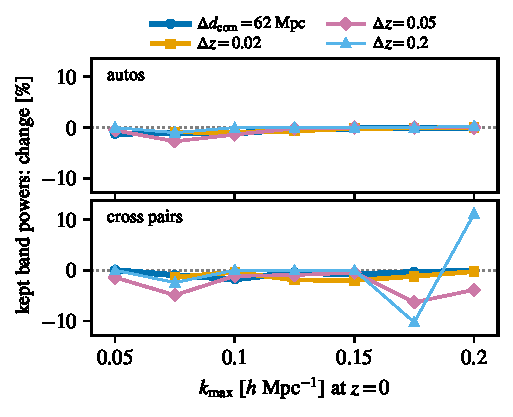
\includegraphics[width=3.5in]{plots/cut_kept_kmax/cut_kept_kmax.pdf}
  \caption{Change of the band powers kept by the UV-fraction scale
    cut when its fiducial becomes the paper model's instead of the
    linear-bias one, for the clustering autos (top) and the
    cross-bin pairs (bottom), per layout (color, line width and
    marker; legend).  The dotted line marks no change.  Every count
    intersects the cut with the shipped mask; $\Delta z = 0.02$
    keeps no band at $0.05\hMpc$.  \kmaxclause}
  \label{fig:kept}
\end{figure}

\begin{table}[tbp]
  \centering
  \begin{tabular}{lccc}
    \hline
    layout & $\kmax = 0.075\hMpc$ & $0.1$ & $0.2$ \\
    \hline
    \dcom{}           & $-1.0\%$ & $-1.4\%$ & $-0.1\%$ \\
    $\Delta z = 0.02$ & $-1.1\%$ & $-0.6\%$ & $-0.2\%$ \\
    $\Delta z = 0.05$ & $-3.2\%$ & $-1.3\%$ & $-2.0\%$ \\
    $\Delta z = 0.2$  & $-1.4\%$ & $+0.0\%$ & $+5.5\%$ \\
    \hline
  \end{tabular}
  \caption{Change of the kept band powers (cut intersected with the
    shipped mask), linear-bias cut to paper-fiducial cut.
    \kmaxclause}
  \label{tab:kept}
\end{table}

\paragraph{Fragile cross pairs.}
The cross pairs move both ways, by one band at
$\kmax \le 0.1\hMpc$.  At $0.175$ and above on the wider layouts, a
handful of adjacent pairs swing by tens of bands: these are spectra
that change sign along $\ell$, so $|C_\ell|$ passes near zero, the
UV fraction crosses $\auv$ at a low band, and the prefix rule then
removes everything after it.  A percent-level change of the model
moves that crossing by many bands in either direction -- the
$+5.5\%$ of $\Delta z = 0.2$ at $0.2\hMpc$ is one such pair keeping
$36$ bands instead of $3$.  The linear-bias cut of these pairs is
exactly as fragile as the paper-fiducial one; neither is better
defined.

\paragraph{The science.}
Figure~\ref{fig:fom} shows what the moved bands are worth.  On the
main layouts the paper model's figures of merit under the
paper-fiducial cut are $0.95$--$1.00$ of their values under the
linear-bias cut: $1$--$3\%$ lower on the thin layouts at every cut,
with the largest single cost $5.3\%$ in ${\rm FoM}(w_0, w_a)$ and
$6.4\%$ in ${\rm FoM}(\Omega_m, 10^9 A_{\rm s})$ on
$\Delta z = 0.05$ at $0.1\hMpc$.  The honesty of the fit does not
move: $\eta = \sqrt{\langle\chi^2\rangle/n_{\rm dof}}$, the check
that the quoted error bars cover where the fit lands under the
known drifts plus the prior scatter, stays between $1.000$ and
$1.031$ under both cuts and changes by at most $0.004$; the
coverage of the $68.3\%$ region changes by at most $0.003$.  The
largest change of any tested parameter shift is $0.034\sigma$.  The
break points of the bias tests -- the largest cut at which every
tested truth shifts the fit by less than $\sigma/3$ -- are identical
under both cuts on every layout: no cut moves from pass to fail or
back.

\begin{figure}[tbp]
  \centering
  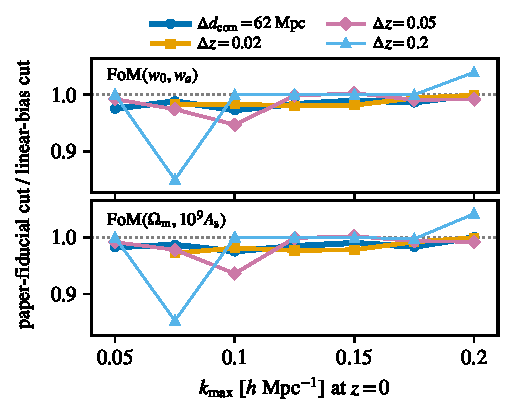
\includegraphics[width=3.5in]{plots/fom_ratio_kmax/fom_ratio_kmax.pdf}
  \caption{The paper model's figures of merit under the
    paper-fiducial cut over those under the linear-bias cut,
    ${\rm FoM}(w_0, w_a)$ (top) and
    ${\rm FoM}(\Omega_m, 10^9 A_{\rm s})$ (bottom), per layout
    (color, line width and marker; legend).  The dotted line marks a
    ratio of one.  $\Delta z = 0.02$ has no fit at $0.05\hMpc$; each
    cut is intersected with the shipped mask.  \kmaxclause}
  \label{fig:fom}
\end{figure}

\paragraph{The one large move.}
The outlier is $\Delta z = 0.2$ at $0.075\hMpc$: the FoM ratio is
$0.85$.  Four bands go there -- one each from a BGS and an LRG3
auto, one from each of two LRG3$\times$ELG1 pairs -- and with ten
wide bins and few bands per bin at that cut, those four carry a
large share of the information ($\sigma(\Omega_m)$ moves from
$0.581$ to $0.671$).  The $+4\%$ of the same layout at $0.2\hMpc$
is the fragile sign-changing pair above, not the bias model.

\paragraph{The adopted choice.}
The forecast computes the cut on the model it analyzes.  The paper
notebook computes its cut on the paper model's fiducial and caches it
(Section~\ref{sec:fiducial}); every Fisher result of the paper model
uses that cache.  The linear-bias notebooks keep the cut computed on
the linear fiducial for the linear experiments.  The numbers of this
section are the price of that consistency: a few percent of either
figure of merit on the main layouts and $15\%$ on the coarse control
at its smallest useful cut, with $\eta$, the coverage and every
pass/fail conclusion unchanged.  The cut cache is tied to
its fiducial: when the fiducial model changes, the cut is recomputed
and the cache replaced.

\section{Attribution: $b_2$ carries the change}
\label{sec:attr}

\paragraph{One term at a time.}
Since the two fiducials differ only through $b_2$ and $b_{s^2}$, the
change can be attributed by switching the two on one at a time:
once with $b_2$ on its calibration and $b_{s^2} = 0$, once the
reverse.  Table~\ref{tab:attr} shows the moved bands against the
linear-bias cut.  $b_2$ alone reproduces $96$--$100\%$ of the change
on $\Delta z = 0.05$ at $0.075$--$0.1\hMpc$ and $67$--$77\%$ on
\dcom{}; $b_{s^2}$ alone moves at most four bands anywhere.  The
remainder is non-additive and comes from the $b_2$--$b_{s^2}$ cross
terms -- the $b_2 b_{s^2}$ loop and the cross part of
$P_\infty \propto (b_2 + \tfrac{2}{3} b_{s^2})^2$.

\begin{table}[tbp]
  \centering
  \begin{tabular}{lcccc}
    \hline
    & \multicolumn{2}{c}{\dcom{}} &
      \multicolumn{2}{c}{$\Delta z = 0.05$} \\
    kept bands moved by & $0.075\hMpc$ & $0.1$ & $0.075$ & $0.1$ \\
    \hline
    $b_2$ alone        & $-12$ & $-30$ & $-26$ & $-16$ \\
    $b_{s^2}$ alone    & $-1$  & $-4$  & $-1$  & $-1$  \\
    both (paper fiducial) & $-18$ & $-39$ & $-27$ & $-16$ \\
    \hline
  \end{tabular}
  \caption{Kept band powers moved against the linear-bias cut when
    each second-order bias is switched on alone, and when both are
    (the paper fiducial).  \kmaxclause}
  \label{tab:attr}
\end{table}

\section{Robustness: the cut within the bias priors}
\label{sec:robust}

\paragraph{Three shifted fiducials.}
The paper fiducial is one point; the analysis samples around it.
Three coherent shifts of the paper fiducial, each at the scale its
own prior allows, measure how stable the cut is inside that volume
(all numbers at $0.075$--$0.1\hMpc$ on \dcom{} and
$\Delta z = 0.05$, kept band powers against the paper-fiducial
cut):
\begin{enumerate}
  \item \textbf{Linear bias up $6\%$} ($+2$ widths of the
    pessimistic prior's per-bin residual, with $b_2$ and $b_{s^2}$
    following their calibrations): the cut keeps $+1.0$ to $+2.1\%$
    more.
  \item \textbf{The $b_2$ and $b_{s^2}$ offsets at $\pm 2$ prior
    widths} ($\Delta_2 = \pm 4$ and $\Delta_s = \pm 2$ in every
    group, the fiducial model's sampling freedom around the
    calibrations):
    the cut keeps $19$--$35\%$ \emph{fewer} band powers, under
    either sign.  A $b_2$ four units off its calibration makes the
    loop terms a large share of $P_{gg}$ near the threshold, so the
    UV fraction rises everywhere.
  \item \textbf{The counterterm $\alpha_0$ at $+1$ prior width}
    ($+16.1\aunit$): the cut keeps $1.9$--$3.7\%$ fewer.  A
    $k^2 P$ term is pure UV-weighted power; this one shift, inside
    one prior width, moves the cut as much as the whole
    linear-to-paper change does.
\end{enumerate}

\paragraph{Against what the data constrain.}
These are not academic excursions.  At the cuts where the bias tests
pass or nearly pass, the data barely measure the offsets: the paper
model's marginalized errors on $\Delta_2$ are $1.4$--$2.0$ at
$0.075\hMpc$ and $0.9$--$1.9$ at $0.1$, close to the prior width
$2$.  An offset of $4$ is therefore a plausible $2\sigma$ posterior
excursion, and within it the cut moves ten to thirty times more
than between the linear-bias and paper fiducials.  Both fiducials
are points inside that band.

\paragraph{Caveats.}
The shifts are rigid: every group moves together, by a prior-width
multiple, which is rarer than a posterior draw of the same size; and
nothing is refitted, so the quoted band-power changes measure the
cut's sensitivity, not a constraint.  The conclusion they support is
deliberately limited: the choice between the two fiducials is a
small effect \emph{compared with} the cut's dependence on where the
bias parameters actually sit.

\appendix

\section{Method and checks}
\label{app:method}

\paragraph{The cuts.}
Each cut is the project's own scale-cut call
(\texttt{gg\us scale\us cuts\us tomo}, the binding of
\texttt{cosmolike/cosmo2D\us scuts.c}) run at the scale-cut study's
reference settings, once per fiducial; only the parameter point
changes between runs.  Each run is validated in two ways: its
unwindowed spectra equal the evaluated data vector bitwise on every
shipped entry, and the linear-bias run equals the cached cut of the
linear-bias Fisher results on every kept row of every layout --
settings noise flips at most one band of the cut alone, and never a
kept row.

\paragraph{The scoring.}
The paper model is rescored with the Fisher notebook's own code: the
paper model's derivative base at the final tier (five-point
stencils) and the same covariance, with only the kept rows exchanged.
A different cut selects rows of the cached derivative matrices;
nothing is recomputed, and every row a new mask keeps is checked to
carry a nonzero fiducial entry and derivative row.  On the
paper-fiducial masks the scoring reproduces the paper notebook's
figures of merit (\texttt{notes/bias\us model\us summary}) on every
layout and cut except $\Delta z = 0.2$ at $\kmax = 0.075\hMpc$, where
the notebook's final-tier cut keeps one band that this study's
reference-settings masks cut.
$\eta$, the coverage and the break rule are the builder's own
(known drifts plus the pessimistic prior scatter; a cut passes
while every tested truth shifts the fit by less than $\sigma/3$).

\section{Open issues}
\label{app:open}

\begin{itemize}
  \item \textbf{What the $b_2$ dependence implies.}  Within the
    $b_2$ offsets' own posterior the cut moves ten to thirty times
    more than between the two fiducials: the cut is a convention
    anchored at a parameter point, not a quantity the data pin
    down.  Three responses are possible, each with a cost.  Treat
    the fiducial cut as a fixed convention, like any other fiducial
    choice -- simplest, but the kept data vector would have looked
    substantially different had the fiducial $b_2$ been drawn
    elsewhere in its posterior.  Verify the headline results under
    cuts computed at shifted $b_2$ -- bounded extra work, and this
    note's machinery does it, but it multiplies the cut caches.  Or
    fold the cut's variation into a systematic budget -- the most
    conservative, at the price of wider errors.  The shifts tested
    here are rigid, coherent prior-width excursions; a
    posterior-draw version of the same test would sharpen the
    factor of ten to thirty before any of these responses is
    chosen.
\end{itemize}

\begin{thebibliography}{9}

\bibitem{Saraivanov2026}
E.~Saraivanov, H.~Rubira, V.~Miranda and T.~Eifler,
``Towards the Two-Loop EFTofLSS in Galaxy Lensing Surveys'',
2026, arXiv:2603.13031.

\bibitem{FangKEM2020}
X.~Fang, E.~Krause, T.~Eifler and N.~MacCrann,
``Beyond Limber: efficient computation of angular power spectra for
galaxy clustering and weak lensing'',
2020, arXiv:1911.11947.

\bibitem{Maus2024}
M.~Maus, S.~Chen, M.~White et al.,
``An analysis of parameter compression and full-modeling techniques
with Velocileptors for DESI 2024 and beyond'',
2024, arXiv:2404.07312.

\bibitem{Lazeyras2016}
T.~Lazeyras, C.~Wagner, T.~Baldauf and F.~Schmidt,
``Precision measurement of the local bias of dark matter halos'',
JCAP 02 (2016) 018, arXiv:1511.01096.

\bibitem{DeRoseChen2025}
J.~DeRose and S.~Chen,
``The Lensing Counter Narrative: An Effective Description of
Small-Scale Clustering in Weak Lensing Power Spectra'',
2025, arXiv:2510.18981.

\bibitem{Baldauf2012}
T.~Baldauf, U.~Seljak, V.~Desjacques and P.~McDonald,
``Evidence for quadratic tidal tensor bias from the halo
bispectrum'',
Phys. Rev. D 86, 083540 (2012), arXiv:1201.4827.

\end{thebibliography}

\end{document}
